\documentclass{article}
\usepackage{amsmath} % For align*
\usepackage{amsfonts} % For open face letters
\usepackage{bookmark} % For links
\usepackage{esint} % For contour integrals
\usepackage{float} % For the [H] option on figures
\usepackage{graphicx} % For images

\graphicspath{{./images/}}
\hypersetup{
  colorlinks=true,
  linkcolor=blue,
  urlcolor=blue
}

\newcommand{\Arg}{\operatorname{Arg}}
\newcommand{\Ln}{\operatorname{Ln}}
\renewcommand{\Im}{\operatorname{Im}}
\renewcommand{\Re}{\operatorname{Re}}
\renewcommand{\vec}[1]{\boldsymbol{\mathbf{#1}}}

\title{Advanced Engineering Mathematics Complex Analysis by Dennis G. Zill Notes}
\author{Chris Doble}
\date{February 2024}

\begin{document}

\maketitle

\tableofcontents

\setcounter{section}{16}
\section{Functions of a Complex Variable}

\subsection{Complex Numbers}

\begin{itemize}
  \item A \textbf{complex number} is any number of the form \[z = a + i b\] where $a$ and $b$ are real numbers and $i$ is the imaginary unit such that $i^2 = -1$.

  \item The real number $a$ in the above complex number $z$ is called the \textbf{real part} of $z$ and the real number $b$ (not $i b$) is called the \textbf{imaginary part} of $z$.

  \item The real and imaginary parts of a complex number $z$ are denoted $\Re(z)$ and $\Im(z)$, respectively.

  \item A real constant multiple of the imaginary unit, e.g. $6 i$ is called a \textbf{pure imaginary number}.

  \item Two complex numbers are equal if their real and imaginary parts are equal.

  \item The addition and subtraction of complex numbers occur between the real and imaginary parts, e.g. \[(a + b i) + (c + d i) = (a + c) + (b + d) i.\]

  \item The multiplication of complex numbers occurs elementwise as normal, e.g. \[(a + b i) (c + d i) = a c + a d i + b c i - b d.\]

  \item The \textbf{conjugate} of a complex number $z = a + i b$ is \[\overline{z} = a - i b.\]

  \item The division of complex numbers occurs by multiplying the numerator and denominator by the conjugate of the denominator, e.g. \begin{align*}
          \frac{a + b i}{c + d i} & = \frac{(a + b i) (c - d i)}{(c + d i) (c - d i)}              \\
                                  & = \frac{a c - a d i + b c i + b d}{c^2 + d^2}                  \\
                                  & = \frac{a c + b d}{c^2 + d^2} + i \frac{b c - a d}{c^2 + d^2}.
        \end{align*}

  \item Conjugates have several interesting properties: \begin{align*}
          \overline{z_1 + z_2} & = \overline{z_1} + \overline{z_2}        \\
          \overline{z_1 - z_2} & = \overline{z_1} - \overline{z_2}        \\
          \overline{z_1 z_2}   & = \overline{z_1} \, \overline{z_2}       \\
          \frac{z_1}{z_2}      & = \frac{\overline{z_1}}{\overline{z_2}}.
        \end{align*}

  \item The sum and product of a complex number $z = x + i y$ with its conjugate are real numbers \begin{align*}
          z + \overline{z} & = 2 x       \\
          z \overline{z}   & = x^2 + y^2
        \end{align*} while the difference between a complex number and its conjugate is a purre imaginary number \[z - \overline{z} = 2 i y.\]

  \item The above properties let us define \[\Re(z) = \frac{z + \overline{z}}{2} \text{ and } \Im(z) = \frac{z - \overline{z}}{2 i}.\]

  \item The \textbf{complex plane} or \textbf{$z$-plane} is a coordinate system where the horizontal or $x$-axis is called the \textbf{real axis} and the vertical or $y$-axis is called the \textbf{imaginary axis}. Complex numbers can be plotted in this coordinate system by considering their real and imaginary parts an ordered pair corresponding their position.

  \item The \textbf{modulus} or \textbf{absolute value} of a complex number $z = x + i y$ denoted by $|z|$ is the real number \[|z| = \sqrt{x^2 + y^2} = \sqrt{z \overline{z}}.\] This is the distance between $z$ and the origin in the complex plane.

  \item If you consider two numbers in the complex plane as vectors, the length of their sum can't be longer than their individual lengths combined \[|z_1 + z_2| \le |z_1| + |z_2|.\] This extends to any finite sum \[|z_1 + z_2 + \cdots + z_n| \le |z_1| + |z_2| + \cdots + |z_n|\] and is known as the \textbf{triangle inequality}.
\end{itemize}

\subsection{Powers and Roots}

\begin{itemize}
  \item A complex number can be expressed in \textbf{polar form} \[z = (r \cos \theta) + i (r \sin \theta)\] where $r = |z|$ is the nonnegative modulus of $z$ and $\theta = \arg z$ is the \textbf{argument} of $z$ — the angle between $z$ and the positive real axis measured in the counterclockwise direction.

  \item The argument of a complex number $z$ isn't unique as any multiply of $2 \pi$ can be added to it. The \textbf{principle argument} of $z$ denoted $\Arg z$ is the argument of $z$ restricted to the intercal $-\pi \le \Arg z \le \pi$.

  \item Multiplication and division of complex numbers is simpler in polar form. For two complex numbers $z_1 = r_1 (\cos \theta_1 + i \sin \theta_1)$ and $z_2 = r_2 (\cos \theta_2 + i \sin \theta_2)$ we get \begin{align*}
          z_1 z_2         & = r_1 r_2 [\cos (\theta_1 + \theta_2) + i \sin (\theta_1 + \theta_2)]          \\
          \frac{z_1}{z_2} & = \frac{r_1}{r_2} [\cos (\theta_1 - \theta_2) + i \sin (\theta_1 - \theta_2)].
        \end{align*}

  \item The above formulas can be used to find integer powers of a complex number $z$ \[z^n = r^n (\cos n \theta + i \sin n \theta)\] where $n$ is an integer (including negative integers).

  \item \textbf{DeMoivre's formula} is a special case of the above where $r = 1$ so \[z^n = (\cos \theta + i \sin \theta)^n = \cos n \theta + i \sin n \theta.\]

  \item A number $w$ is said to be an \textbf{$\boldsymbol{n}$th root} of a nonzero complex number $z$ if $w^n = z$. The $n$th roots of a nonzero complex number $z = r (\cos \theta + i \sin \theta)$ are \[w_k = r^{1 / n} \left[ \cos \left( \frac{\theta + 2 k \pi}{n} \right) + i \sin \left( \frac{\theta + 2 k \pi}{n} \right) \right]\] where $k = 0, 1, 2, \ldots, n - 1$.

  \item The root $w$ of a complex number $z$ obtained by using the principle argument of $z$ with $k = 0$ is called the \textbf{principle $\boldsymbol{n}$th root} of $z$.

  \item Since the $n$th roots of a complex number have the same modulus they lie on a circle of radius $r^{1 / n}$. The arguments of subsequent roots differ by $2 \pi / n$ so they're also equally spaced around the circle.
\end{itemize}

\subsection{Sets in the Complex Plane}

\begin{itemize}
  \item The points $z = x + i y$ that satisfy the equation \[|z - z_0| = \rho\] for $\rho > 0$ lie on a circle of radius $\rho$ centred at the point $z_0$.

  \item The points $z$ satisfying the inequality $|z - z_0| < \rho$ for $\rho > 0$ lie within, but not on, a circle of radius $\rho$ centered at the point $z_0$. This set is called a \textbf{neighborhood} of $z_0$ or an \textbf{open disk}.

  \item A point $z_0$ is said to be an \textbf{interior point} of a set $S$ of the complex plane if there exists some neighborhood of $z_0$ that lies entirely within $S$.

  \item If every point $z$ of a set $S$ is an interior point, then $S$ is said to be an \textbf{open set}. An example of a set that isn't open is the set of points satisfying the inequality $\Re (z) \ge 0$. This isn't open because it includes the line $\Re (z) = 0$ and no points on that line are interior to the set because, no matter what $\rho$ you choose, some points in the neighborhood have $\Re (z) < 0$.

  \item If every neighborhood of a point $z_0$ contains at least one point that is in a set $S$ and at least one point that is not in $S$, then $z_0$ is said to be a \textbf{boundary point} of $S$.

  \item The \textbf{boundary} of a set $S$ in the complex plane is the set of all boundary points of $S$.

  \item If any pair of points in a set $S$ can be connected by a polygonal line that lies entirely within the set, then $S$ is said to be \textbf{connected}.

  \item An open connected set is called a \textbf{domain}.

  \item A \textbf{region} is a set in the complex plane with all, some, or none of its boundary points. A region containing all of its boundary points is said to be \textbf{closed}.
\end{itemize}

\subsection{Functions of a Complex Variable}

\begin{itemize}
  \item A \textbf{function} $f$ from a set $A$ to a set $B$ is a rule of correspondence that assigns to each element of $A$ one and only one element of $B$.

  \item If $b$ is the element of $B$ assigned to the element $a$ of $A$, $b$ is said to be the \textbf{image} of $a$ and is denoted $b = f(a)$.

  \item The set $A$ is called the \textbf{domain} of $f$.

  \item The set of all images in $B$ is called the \textbf{range} of $f$.

  \item If $A$ is a set of real numbers, $f$ is said to be a \textbf{function of a real variable $\boldsymbol{x}$}.

  \item If $A$ is a set of complex numbers, $f$ is said to be a \textbf{function of a complex varibale $\boldsymbol{z}$} or a \textbf{complex function}.

  \item The image $w$ of a complex number $z$ is \[w = f(z) = u(x, y) + i v(x, y)\] where $u$ and $v$ are the real and imaginary parts of $w$ and are real-valued functions.

  \item Although we cannot draw a graph of a complex function $w = f(z)$ (because it would require a four-dimensional coordinate system), it can be interpreted as a \textbf{mapping} or \textbf{transformation} from the $z$ plane to the $w$ plane.

  \item A complex function may be interpreted as a two-dimensional fluid flow by considering $w = f(z)$ as the fluid velocity vector at the point $z$. In that case, if $x(t) + i y(t)$ is a parametric representation of a particle's position over time then \begin{align*}
          \frac{d x}{d t} & = u(x, y) \\
          \frac{d y}{d t} & = v(x, y)
        \end{align*} and the family of solutions to this system of differential equations are called the \textbf{streamlines} of the flow associated with $f(z)$.
\end{itemize}

\begin{figure}[H]
  \centering
  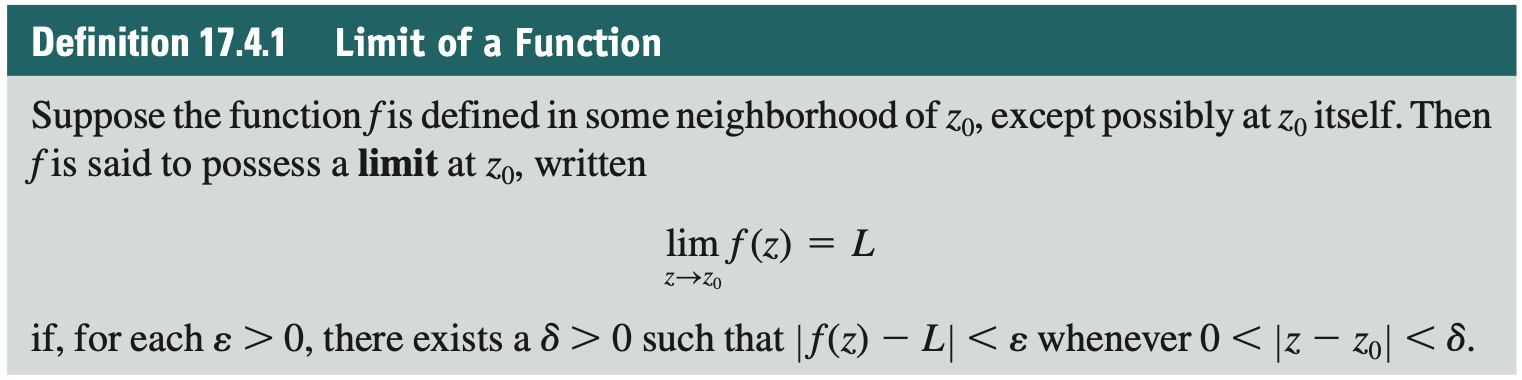
\includegraphics[width=\textwidth]{limit-of-a-function}
\end{figure}

\begin{itemize}
  \item For a function $f$ of a real variable $x$, the limit $\lim_{x \rightarrow x_0} f(x) = L$ means $f$ approaches $L$ as you approach from both the left and right. If however $f$ is a function of a complex variable it means $f$ approaches $L$ as you approach from any direction in the complex plane.
\end{itemize}

\begin{figure}[H]
  \centering
  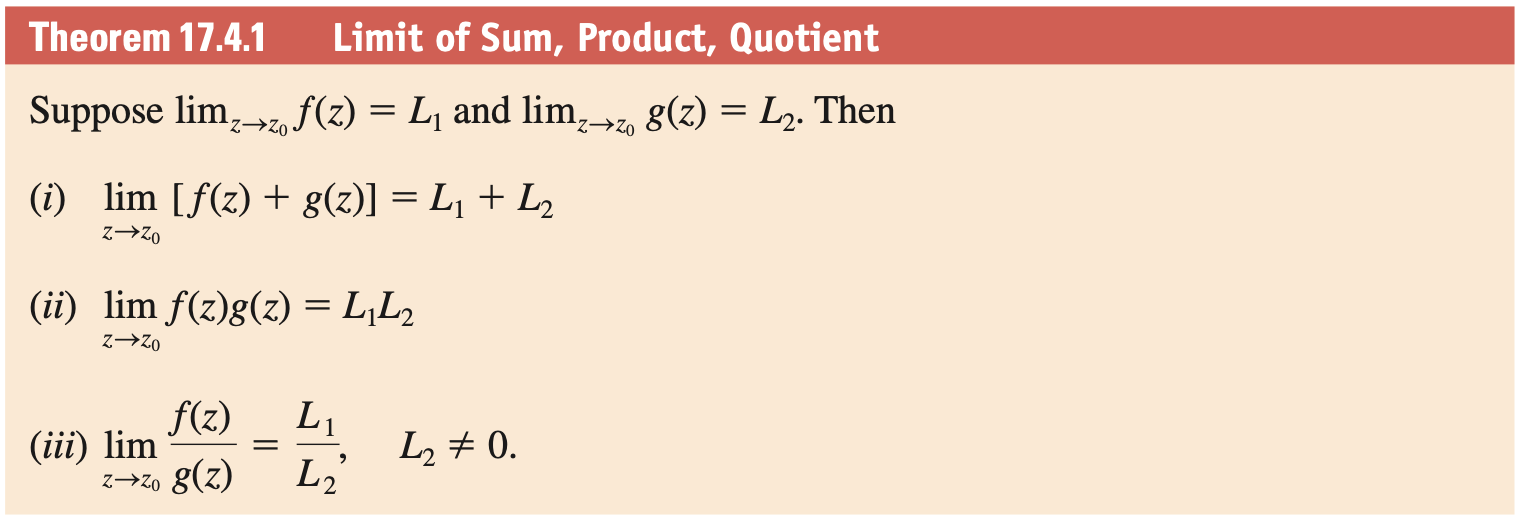
\includegraphics[width=\textwidth]{limit-properties}
\end{figure}

\begin{itemize}
  \item A function $f$ is continuous at a point $z_0$ if \[\lim_{z \rightarrow z_0} f(z) = f(z_0).\]

  \item A function $f$ defined by \[f(z) = a_n z^n + a_{n - 1} z^{n - 1} + \cdots + a_2 z^2 + a_1 z + a_0,\ a_n \ne 0\] where $n$ is a nonnegative integer and the coefficients $a_i$, $i = 0, 1, \ldots, n$, are complex constants is called a \textbf{polynomial} of degree $n$.

  \item Polynomials are continuous on the entire complex plane.

  \item A \textbf{rational function} \[f(z) = \frac{g(z)}{h(z)}\] is continuous everywhere $h(z) \ne 0$.
\end{itemize}

\begin{figure}[H]
  \centering
  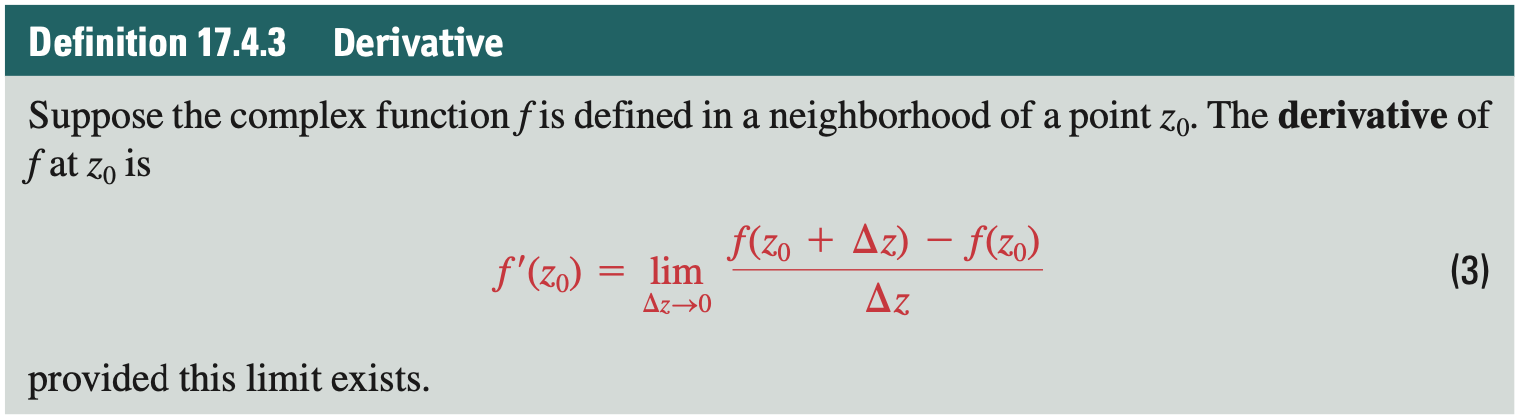
\includegraphics[width=\textwidth]{derivative}
\end{figure}

\begin{itemize}
  \item In order for a complex function to be differentiable, the limit must approach the same value from every direction. This is a greater demand than in real variables. If you take an arbitrary complex function, there's a good chance it isn't differentiable.
\end{itemize}

\begin{figure}[H]
  \centering
  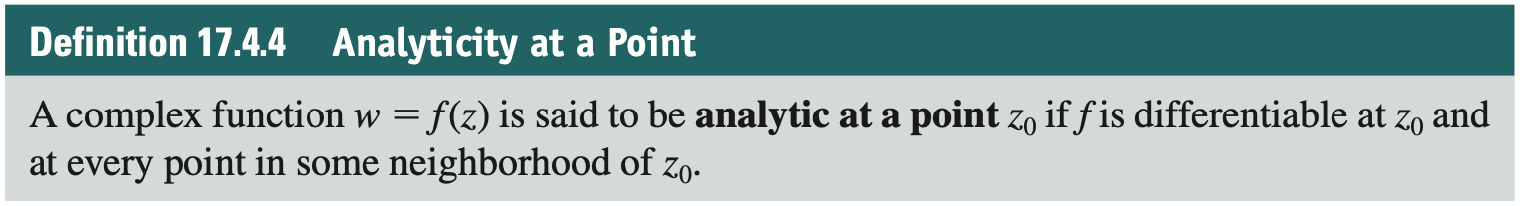
\includegraphics[width=\textwidth]{analyticity}
\end{figure}

\begin{itemize}
  \item Analyticity at a point is a neighborhood property. A function can be differentiable at a point but if the neighboring points aren't also differentiable, it's not analytic at that point.
  
\item A function is analytic in a domain $D$ if it is analytic at every point in $D$.

  \item A function that is analytic everywhere is called an \textbf{entire function}.
\end{itemize}

\subsection{Cauchy-Riemann Equations}

\begin{figure}[H]
  \centering
  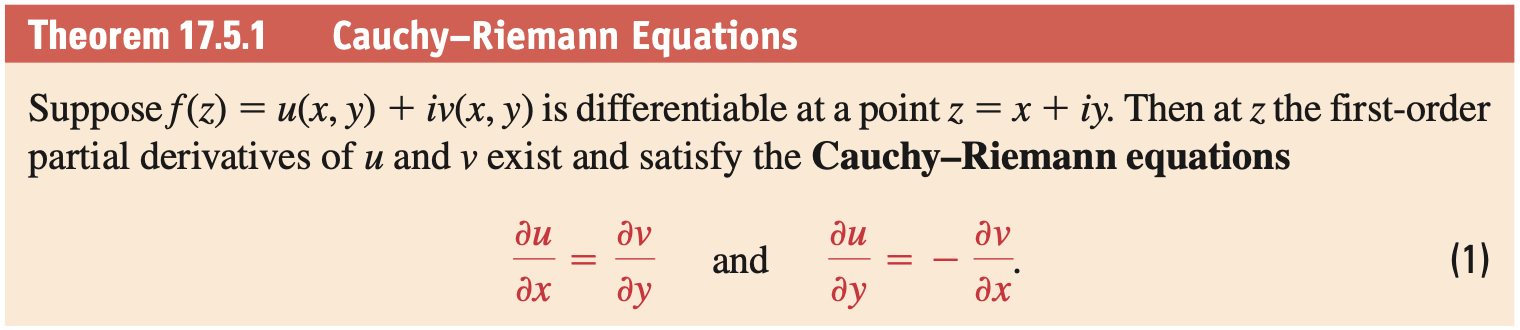
\includegraphics[width=\textwidth]{cauchy-riemann-equations}
\end{figure}

\begin{itemize}
  \item If a complex function $f(z) = u(x, y) + i v(x, y)$ is analytic throughout a domain $D$, then the real functions $u$ and $v$ must satisfy the Cauchy-Riemann equations at every point in $D$.
\end{itemize}

\begin{figure}[H]
  \centering
  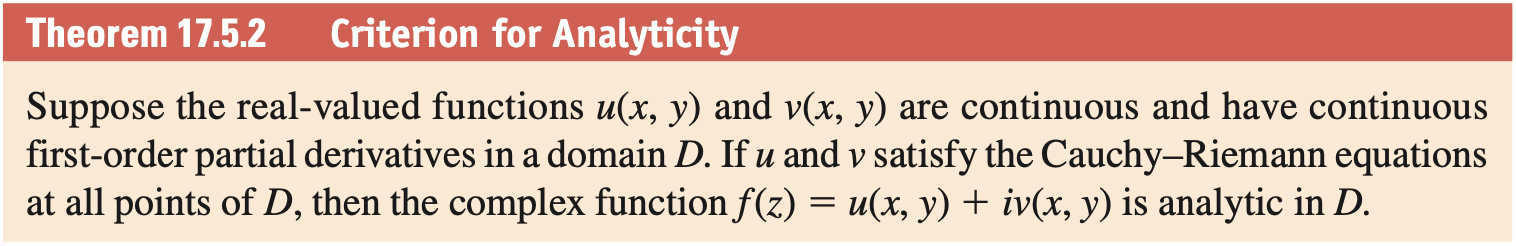
\includegraphics[width=\textwidth]{criterion-for-analyticity}
\end{figure}

\begin{itemize}
  \item The Cauchy-Riemann equations are derived assuming the function is differentiable at a particular point. That being the case, they can also be used as a formula for the derivative of the function \[f'(z) = \frac{\partial u}{\partial x} + i \frac{\partial v}{\partial x} = \frac{\partial v}{\partial y} - i \frac{\partial u}{\partial y}.\]

  \item Because analyticity implies differentiability, theorem 17.5.2 can also be used to determine if a function is differentiable at a point.

  \item A real-valued function $\phi(x, y)$ that has continuous second-order partial derivatives in a domain $D$ and satisfies Laplace's equation is said to be \textbf{harmonic} in $D$.

  \item If a function $f(z) = u(x, y) + i v(x, y)$ is analytic in a domain $D$ then the functions $u(x, y)$ and $v(x, y)$ are harmonic functions.

  \item If a given function $u(x, y)$ is harmonic in a domain $D$ it is sometimes possible to find another function $v(x, y)$ that is harmonic in $D$ such that $u(x, y) + i v(x, y)$ is analytic in $D$. The function $v$ is called the \textbf{harmonic conjugate function} of $u$.

  \item To find the harmonic conjugate function of a given function $u$:

        \begin{enumerate}
          \item Take the first-order partial derivatives of $u$ with respect to $x$ and $y$.

          \item If $u(x, y) + i v(x, y)$ is analytic in a domain $D$ then $u$ and $v$ must satisfy the Cauchy-Riemann equations in $D$ from which we can find expressions for $\partial v / \partial x$ and $\partial v / \partial y$.

          \item Integrate $\partial v / \partial x$ with respect to $x$ to get an expression for $v$ with an unknown constant $h(y)$.

          \item Take the first-order partial derivative of $v$ with respect to $y$, equate it with the other expression for $\partial v / \partial y$, and solve for $h'(y)$.

          \item Integrate $h'(y)$ and substitute the result to find $v$.
        \end{enumerate}
\end{itemize}

\subsection{Exponential and Logarithmic Functions}

\begin{itemize}
  \item The exponential function for complex numbers is defined as \[e^z = e^{x + i y} = e^x (\cos y + i \sin y).\]

  \item $e^z$ is analytic for all $z$, i.e. it's an entire function.

  \item Like its real-valued counterpart, \begin{align*}
          \frac{d}{d z} e^z & = e^z,           \\
          e^{z_1} e^{z_2}   & = e^{z_1 + z_2},
        \end{align*} and \[\frac{e^{z_1}}{e^{z_2}} = e^{z_1 - z_2}.\]

  \item Since \[e^{2 \pi i} = \cos (2 \pi) + i \sin (2 \pi) = 1\] and \[e^{z + 2 \pi i} = e^z e^{2 \pi i} = e^z\] the complex function $f(z) = e^z$ is \textbf{periodic} with complex period $2 \pi i$. Because of this complex periodicity an infinite horizontal strip of height $2 \pi$ contains all possible values for the function. The strip $-\pi < y \le \pi$ is called the \textbf{fundamental region}.

  \item For $z \ne 0$ and $\theta = \arg z$, \[\ln z = \log_e |z| + i (\theta + 2 n \pi),\ n = 0, \,\pm 1, \,\pm 2, \,\ldots\] This means there are infinitely many values of the logarithm of a complex number $z$. This makes sense as the complex exponential is periodic.

  \item The \textbf{principal value} of $\ln z$ is the complex logarithm corresponding to $n = 0$ and $\theta = \Arg z$. It is denoted $\Ln z$.

  \item Some familiar properties of the real-valued logarithm hold for the complex-valued logarithm, e.g. \[\ln (z_1 z_2) = \ln z_1 + \ln z_2\] and \[\ln \left( \frac{z_1}{z_2} \right) = \ln z_1 - \ln z_2,\] however they don't necessarily hold for the principal value.

  \item $\Ln z$ is discontinuous and thus not analytic at $z = 0$ because $\ln z$ is undefined at $z = 0$ and on the negative real axis because $\Arg z$ is discontinuous there.

  \item The derivative of $\Ln z$ is \[\frac{d}{d z} \Ln z = \frac{1}{z}.\]

  \item The complex power of a complex number is defined as \[z^\alpha = e^{\alpha \ln z}, \ z \ne 0.\] In general this is multiple-valued because $\ln z$ is multiple-valued — only if $\alpha = n,\ n = 0, \ \pm 1, \,\pm 2, \,\ldots$ is it single-valued. If $\ln z$ is replaced with $\Ln z$ then we get the \textbf{principle value} of $z^\alpha$.
\end{itemize}

\subsection{Trigonometric and Hyperbolic Functions}

\begin{figure}[H]
  \centering
  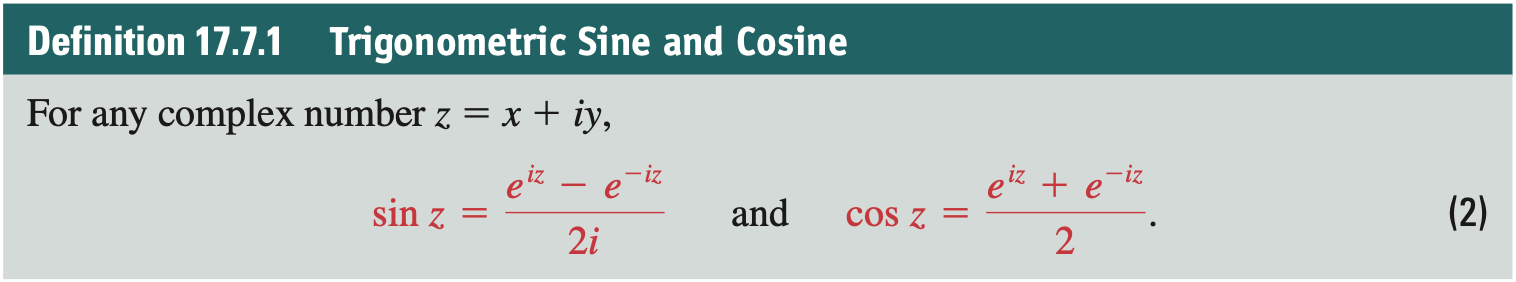
\includegraphics[width=\textwidth]{sine-and-cosine}
\end{figure}

\begin{itemize}
  \item The other trigonometric functions ($\tan z$, etc.) are defined as usual.

  \item Because $e^{i z}$ and $e^{-i z}$ are entire functions, $\sin z$ and $\cos z$ are also entire functions.

  \item $\sin z = 0$ for the real numbers $z = n \pi, \,n \in \mathbb{Z}$ and $\cos z = 0$ for the real numbers $z = (2 n + 1) \pi / 2, \,n \in \mathbb{Z}$. This means that $\tan z$ and $\sec z$ are analytic except at the points where $\cos z = 0$ and $\cot z$ and $\sec z$ are analytic except at the points where $\sin z = 0$.

  \item The usual derivatives and trigonometric functions are still valid in the complex case.

  \item $\sin z$ can be expressed as \[\sin z = \sin x \cosh y + i \cos x \sinh y\] and $\cos z$ can be expressed as \[\cos z = \cos x \cosh y - i \sin x \sinh y.\]

  \item The only zeroes of $\sin z$ are the real numbers $z = n \pi, \,n \in \mathbb{Z}$ and the only zeroes of $\cos z$ are the real numbers $z = (2 n + 1) \pi / 2, \,n \in \mathbb{Z}$.
\end{itemize}

\begin{figure}[H]
  \centering
  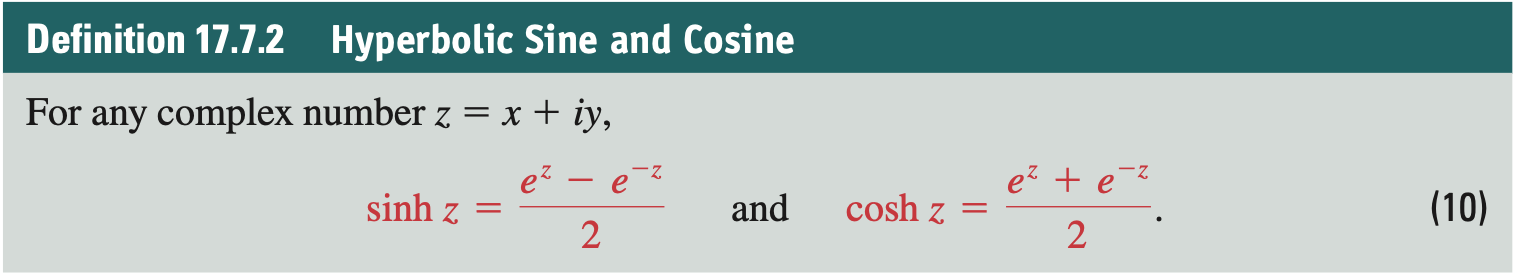
\includegraphics[width=\textwidth]{hyperbolic-sine-and-cosine}
\end{figure}

\begin{itemize}
  \item The complex trigonometric functions can be expressed in terms of the complex hyperbolic functions and vice versa \begin{align*}
          \sin z  & = -i \sinh (i z), & \cos z  & = \cosh (i z) \\
          \sinh z & = -i \sin (i z),  & \cosh z & = \cos (i z).
        \end{align*}

  \item $\sinh z$ can be expressed as \[\sinh z = \sinh x \cos y + i \cosh x \sin y\] and $\cosh z$ can be expressed as \[\cosh z = \cosh x \cos y + i \sinh x \sin y.\]

  \item The zeroes of $\sinh z$ are $z = n \pi i, \,n \in \mathbb{Z}$ and the zeroes of $\cosh z$ are $z = (2 n + 1) \pi i / 2, \,n \in \mathbb{Z}$.

  \item $\sin z$ and $\cos z$ are $2 \pi$ periodic while $\sinh z$ and $\cosh z$ are $2 \pi i$ periodic.
\end{itemize}

\subsection{Inverse Trigonometric and Hyperbolic Functions}

\begin{itemize}
  \item Because the complex trigonometric functions are multi-valued, their inverse functions are also multi-valued.

  \item The definitions of those inverse functions are \begin{align*}
          \arcsin z & = -i \ln [i z + (1 - z^2)^{1 / 2}],             \\
          \arccos z & = -i \ln [z + i (1 - z^2)^{1 / 2}], \text{ and} \\
          \arctan z & = \frac{i}{2} \ln \frac{i + z}{i - z}.
        \end{align*}

  \item The derivatives of the inverse trigonometric functions are \begin{align*}
          \frac{d}{d z} \arcsin z & = \frac{1}{(1 - z^2)^{1 / 2}},              \\
          \frac{d}{d z} \arccos z & = \frac{-1}{(1 - z^2)^{1 / 2}}, \text{ and} \\
          \frac{d}{d z} \arctan z & = \frac{1}{1 + z^2}.
        \end{align*}

  \item The definitions of the hyperbolic inverse functions and their derivatives are

        \begin{figure}[H]
          \centering
          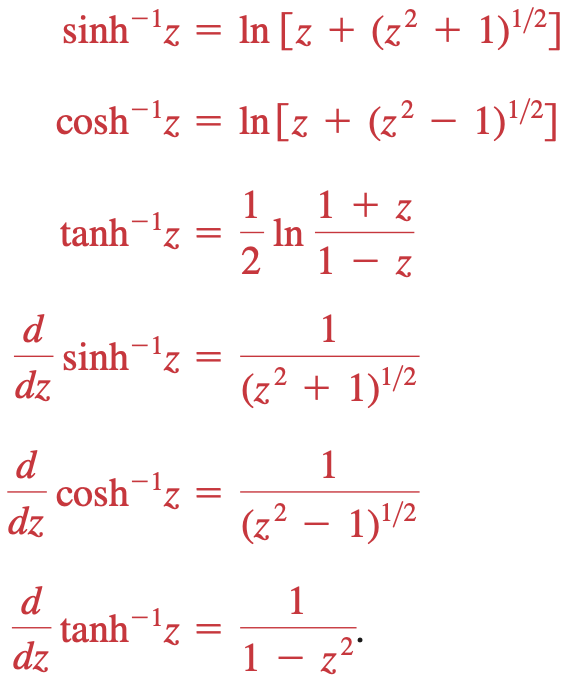
\includegraphics[width=0.4 \textwidth]{inverse-hyperbolic-functions}
        \end{figure}
\end{itemize}

\section{Integration in the Complex Plane}

\subsection{Contour Integrals}

\begin{itemize}
  \item In complex variables, a piecewise smooth curve $C$ is called a \textbf{contour} or \textbf{path}. An integral of a complex function $f(z)$ on $C$ is denoted $\int_C f(z) \,d z$ or $\oint_C f(z) \,d z$ if $C$ is closed — this is called a \textbf{contour integral} or a \textbf{complex integral}.
\end{itemize}

\begin{figure}[H]
  \centering
  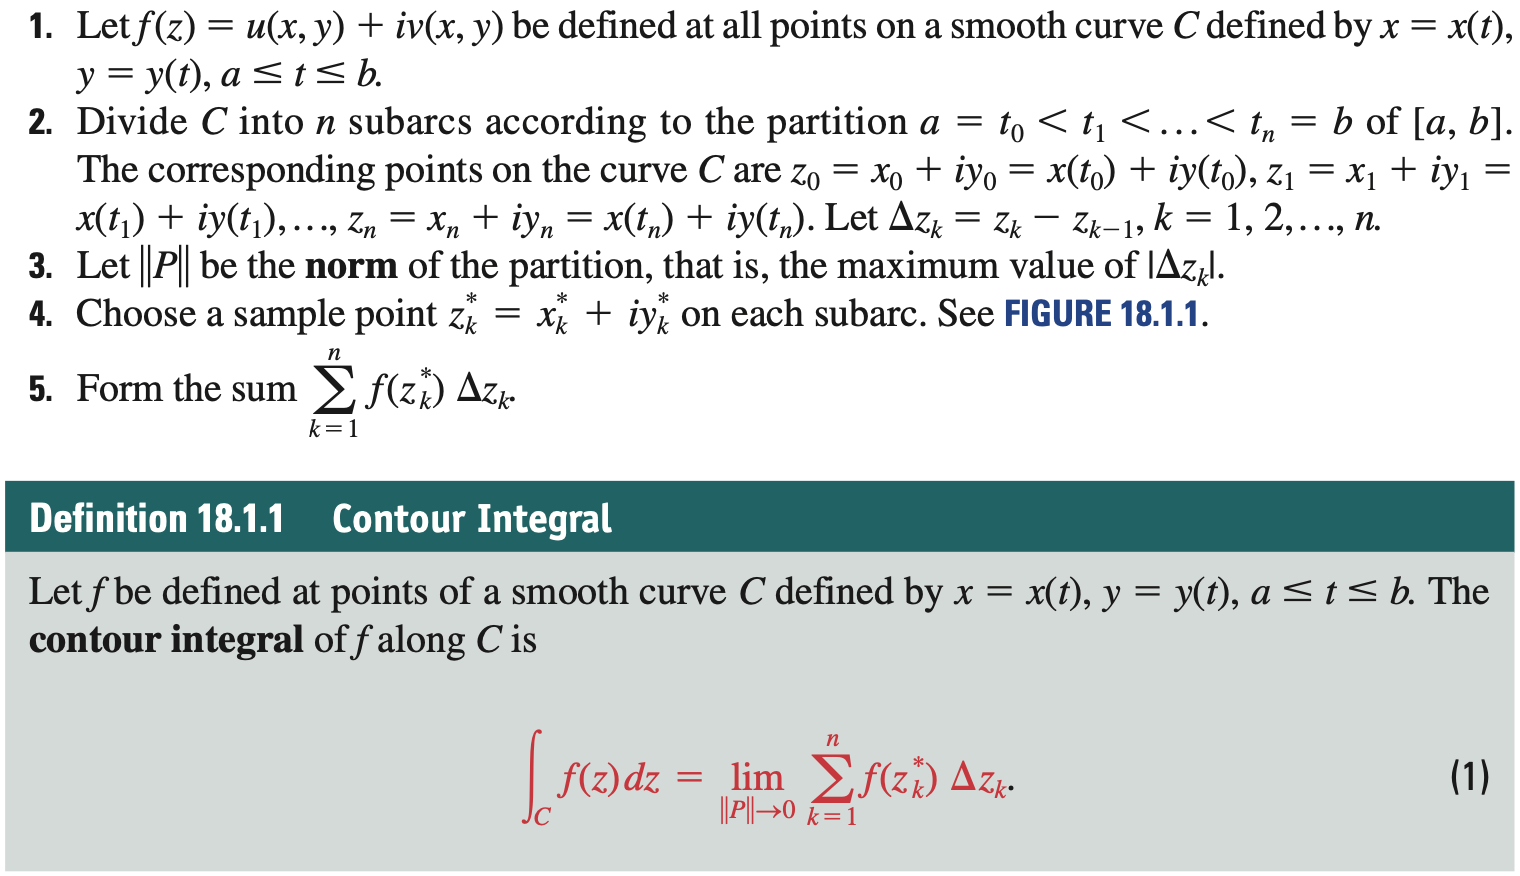
\includegraphics[width=\textwidth]{contour-integral}
\end{figure}

\begin{figure}[H]
  \centering
  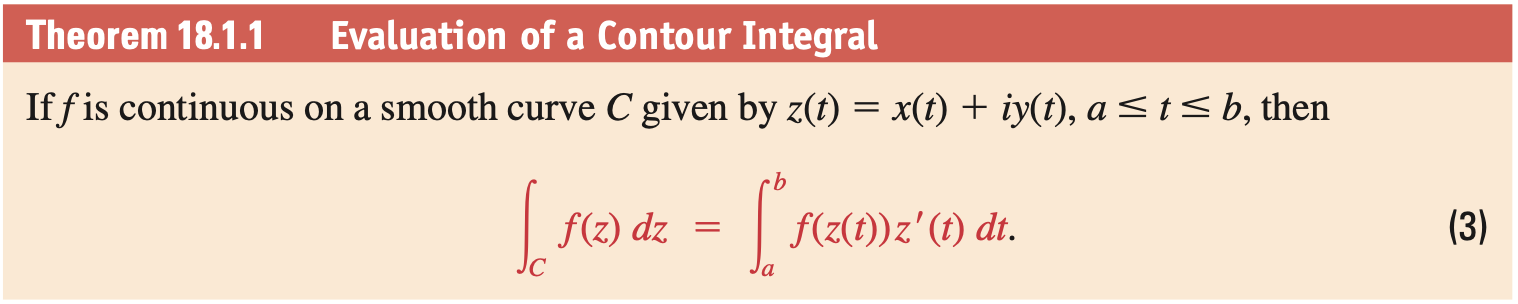
\includegraphics[width=\textwidth]{contour-integral-evaluation}
\end{figure}

\begin{itemize}
  \item If a complex function $f$ is continuous on a smooth curve $C$ and if $|f(z)| \le M$ for all $z$ on $C$, then \[\left| \int_C f(z) \,d z \right| \le M L,\] where \[L = \int_a^b |z'(t)| \,d t\] is the length of $C$. This is sometimes called the \textbf{ML-intequality}.

  \item If $\vec{T}$ is the unit tangent vector to a positively oriented simple closed curve $C$ then \[\varointctrclockwise_C f \cdot \vec{T} \,d s = \Re \left( \varointctrclockwise \overline{f(z)} \,d z \right)\] is called the \textbf{circulation} around $C$ and measures the tendency of the flow to rotate the curve $C$.

  \item If $\vec{N}$ is the normal vector to a positive oriented simple closed curve $C$ then \[\varointctrclockwise_C f \cdot \vec{N} \,d s = \Im \left( \varointctrclockwise \overline{f(z)} \,d z \right)\] is called the \textbf{net flux} across $C$ and measures the difference between the rates at which fluid enters and exits the region bounded by $C$.
\end{itemize}

\subsection{Cauchy-Goursat Theorem}

\begin{itemize}
  \item A domain $D$ is said to be \textbf{simply connected} if every simple closed contour $C$ lying entirely in $D$ can be shrunk to a point without leaving $D$, i.e. the domain has no holes in it.

  \item A domain that is not simply connected is called a \textbf{multiply connected domain}. A domain with one hole is called \textbf{doubly connected}, a domain with two holes \textbf{triply connected}, etc.
\end{itemize}

\begin{figure}[H]
  \centering
  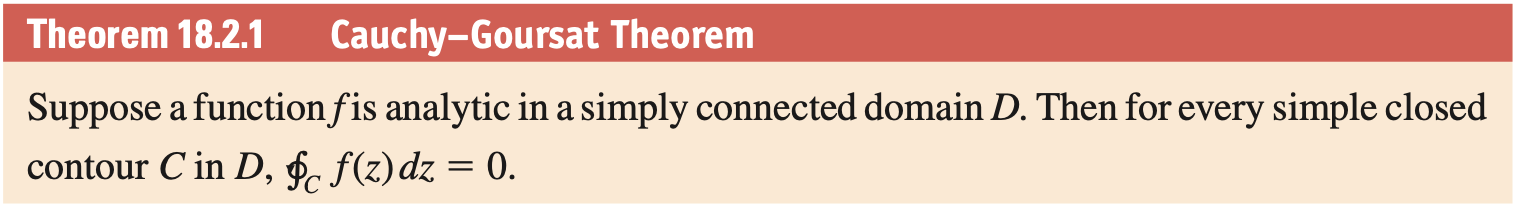
\includegraphics[width=\textwidth]{cauchy-goursat-theorem}
\end{figure}

\begin{itemize}
  \item An alternative way of stating the Cauchy-Goursat Theorem is: if $f$ is analytic at all points on and within a simple closed contour $C$, then $\oint_C f(z) \,d z = 0$.

  \item If $D$ is a double connected domain and $C$ and $C_1$ are simple closed contours such that $C_1$ surrounds the ``hole'' in the domain and is interior to $C$, then \[\varointctrclockwise_C f(z) \,d z = \varointctrclockwise_{C_1} f(z) \,d z.\] This is called the principle of \textbf{deformation of contours} since $C_1$ can be considered a continuous deformation of the contour $C$ (or vice versa) under which the value of the integal doesn't change.

  \item If $z_0$ is a constant complex number interior to a simple closed contour $C$, then \[\varointctrclockwise_C \frac{d z}{(z - z_0)^n} = \begin{cases}
            2 \pi i & n = 1                      \\
            0       & n \text{ an integer} \ne 1
          \end{cases}.\]
\end{itemize}

\begin{figure}[H]
  \centering
  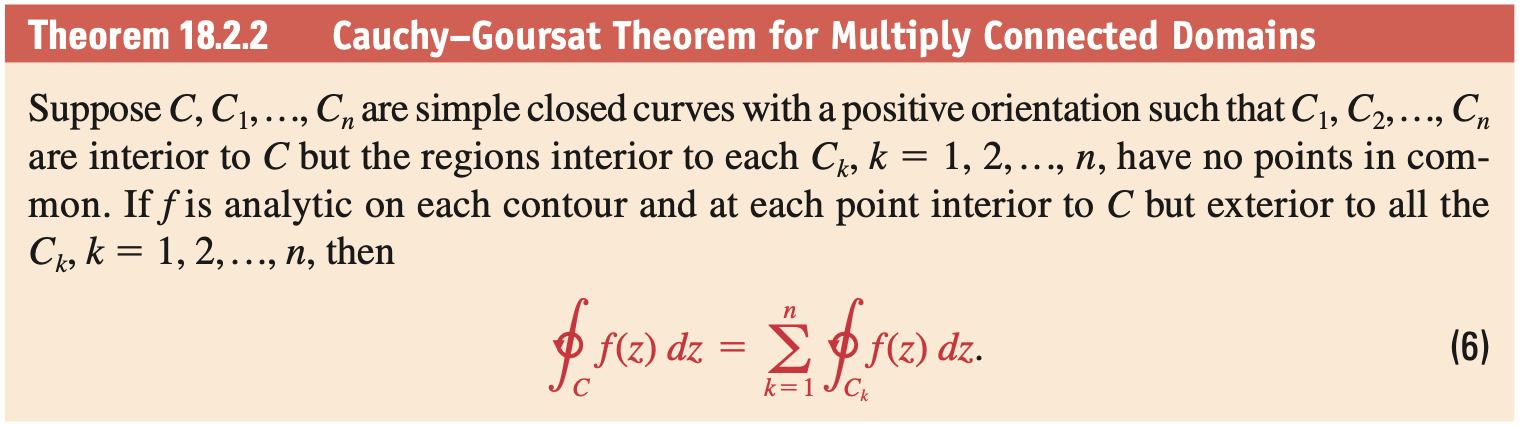
\includegraphics[width=\textwidth]{cauchy-goursat-theorem-multiply-connected-domains}
\end{figure}

\subsection{Independence of the Path}

\begin{itemize}
  \item Let $z_0$ and $z_1$ be points in a domain $D$. A contour integral $\int_C f(z) \,d z$ is said to be \textbf{independent of the path} if its value is the same for all contours $C$ in $D$ with an initial point $z_0$ and a terminal point $z_1$.

  \item If $f$ is an analytic function in a simply connected domain $D$, then \\ $\int_C f(z) \,d z$ is independent of path $C$.

  \item Suppose $f$ is continuous in a domain $D$. If there exists a function $F$ such that $F'(z) = f(z)$ for each $z$ in $D$, then $F$ is called the \textbf{antiderivative} of $f$.

  \item The general antiderivative of a complex function includes a complex integration constant.

  \item Suppose $f$ is continuous in a domain $D$ and $F$ is an antiderivative of $f$ in $D$. Then for any contour $C$ in $D$ with initial point $z_0$ and terminal point $z_1$, \[\int_C f(z) \,d z = F(z_1) - F(z_0).\]

  \item A consequence of the above is that if $C$ is closed, then \[\varointctrclockwise_C f(z) \,d z = 0.\]

  \item If $f$ is analytic in a simply connected domain $D$, then $f$ has an antiderivative in $D$; this, there exists a function $F$ such that $F'(z) = f(z)$ for all $z$ in $D$.

  \item Suppose $f$ and $g$ are analytic in a simply connected domain $D$ that contains the contour $C$. If $z_0$ and $z_1$ are the initial and terminal points of $C$, then the \textbf{integration by parts} formula is valid in $D$: \[\int_{z_0}^{z_1} f(z) g'(z) \,d z = f(z) g(z)|_{z_0}^{z_1} - \int_{z_0}^{z_1} f'(z) g(z) \,d z.\]
\end{itemize}

\subsection{Cauchy's Integral Formulas}

\begin{figure}[H]
  \centering
  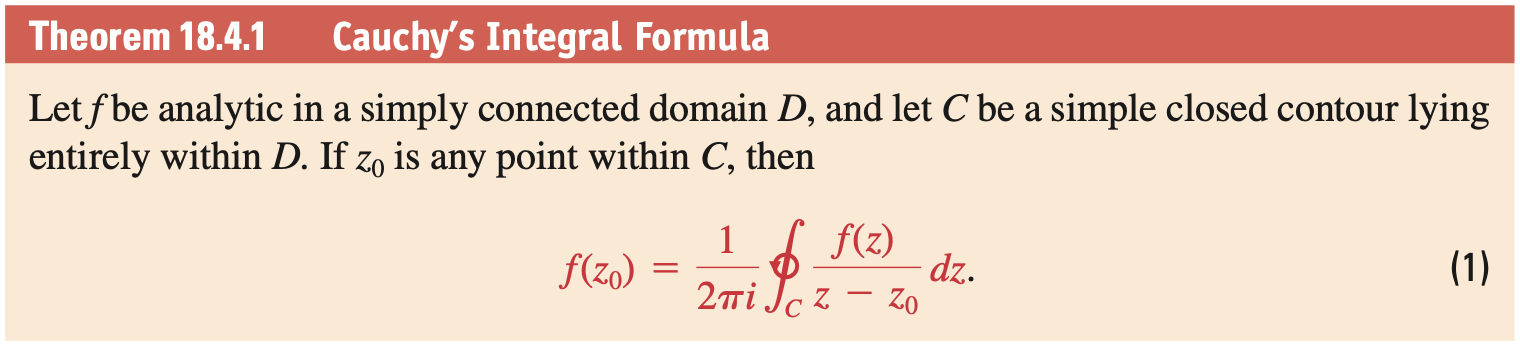
\includegraphics[width=\textwidth]{cauchys-integral-formula}
\end{figure}

\begin{itemize}
  \item Cauchy's integral formula is useful when a contour integral has the form \[\varointctrclockwise \frac{f(z)}{z - z_0} \,d z\] in which case you know its value is $2 \pi i f(z_0)$.
\end{itemize}

\begin{figure}[H]
  \centering
  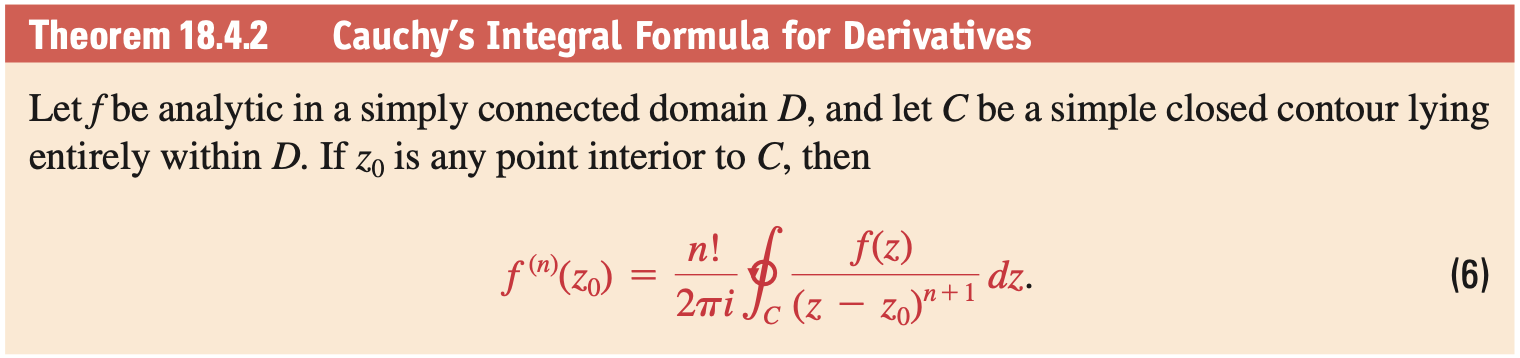
\includegraphics[width=\textwidth]{cauchys-integral-formula-for-derivatives}
\end{figure}

\begin{itemize}
  \item Cauchy's integral formula for derivatives is useful when a contour integral has the form \[\varointctrclockwise \frac{f(z)}{(z - z_0)^{n + 1}} \,d z\] in which case you know its value is $\frac{2 \pi i}{n!} f^{(n)}(z_0)$.

  \item \textbf{Liouville's theorem} states that the only bounded entire functions are constants.
\end{itemize}

\section{Series and Residues}

\subsection{Sequences and Series}

\begin{itemize}
  \item A \textbf{sequence} is a function whose domain is the set of positive integers, i.e. for each integer $n = 1, 2, 3, \ldots$ we assign a complex number $z_n$.

  \item If $\lim_{n \rightarrow \infty} z_n = L$ we say the sequence $\{ z_n \}$ is \textbf{convergent}. In otherwords, $\{ z_n \}$ converges to the number $L$ if, for every positive number $\varepsilon$, an $N$ can be found such that $|z_n - L| < \varepsilon$ whenever $n > N$.

  \item A sequence $\{ z_n \}$ converges to a complex number $L$ if and only if $\Re (z_n)$ converges to $\Re (L)$ and $\Im (z_n)$ converges to $\Im (L)$.

  \item An \textbf{infinite series} of complex numbers \[\sum_{k = 1}^\infty z_k = z_1 + z_2 + \cdots\] is \textbf{convergent} if the sequence of partial sums $\{ S_n \}$, where \[S_n = z_1 + z_2 + \cdots + z_n\] converges. If $S_n \rightarrow L$ as $n \rightarrow \infty$, we say that the \textbf{sum} of the series is $L$.

  \item The sum of the geometric series \[\sum_{k = 1}^\infty a z^{k - 1} = a + a z + a z^2 + \cdots\] converges to \[\frac{a}{1 - z}\] when $|z| < 1$ and diverges otherwise.

  \item If $\sum_{k = 1}^\infty z_k$ converges, then $\lim_{n \rightarrow \infty} z_n = 0$.

  \item If $\lim_{n \rightarrow \infty} z_n \ne 0$ then the series $\sum_{k = 1}^\infty z_k$ diverges.

  \item An infinite series $\sum_{k = 1}^\infty z_k$ is said to be \textbf{absolutely convergent} if \\ $\sum_{k = 1}^\infty |z_k|$ converges. Absolute convergence implies convergence.
\end{itemize}

\begin{figure}[H]
  \centering
  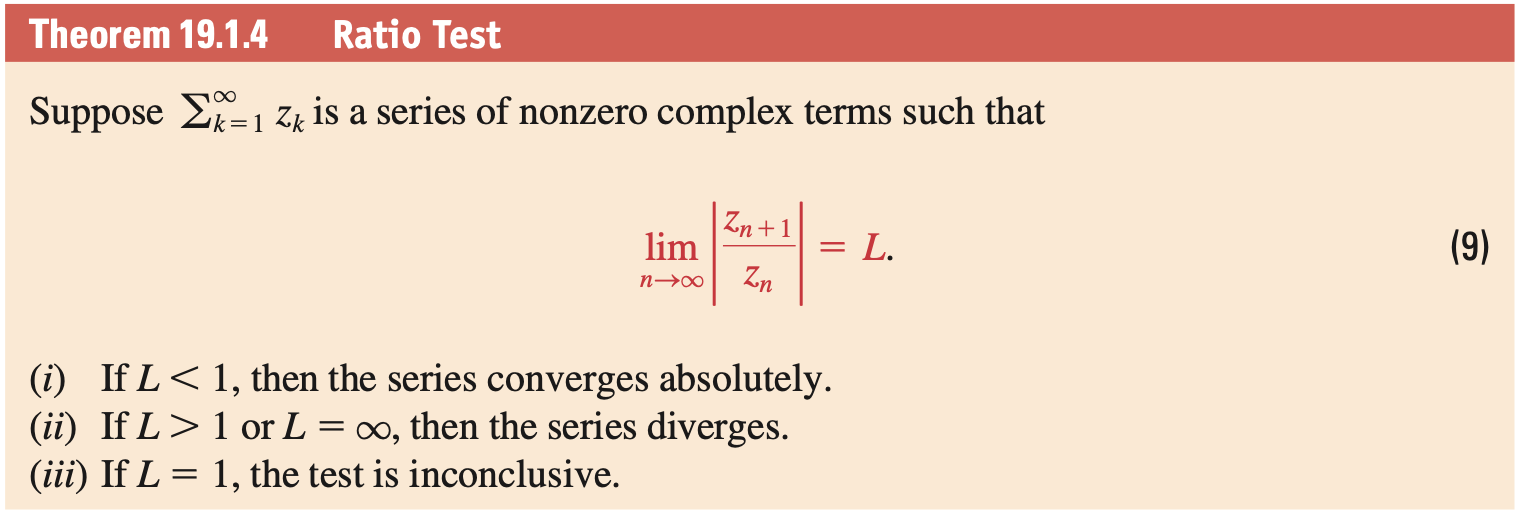
\includegraphics[width=\textwidth]{ratio-test}
\end{figure}

\begin{figure}[H]
  \centering
  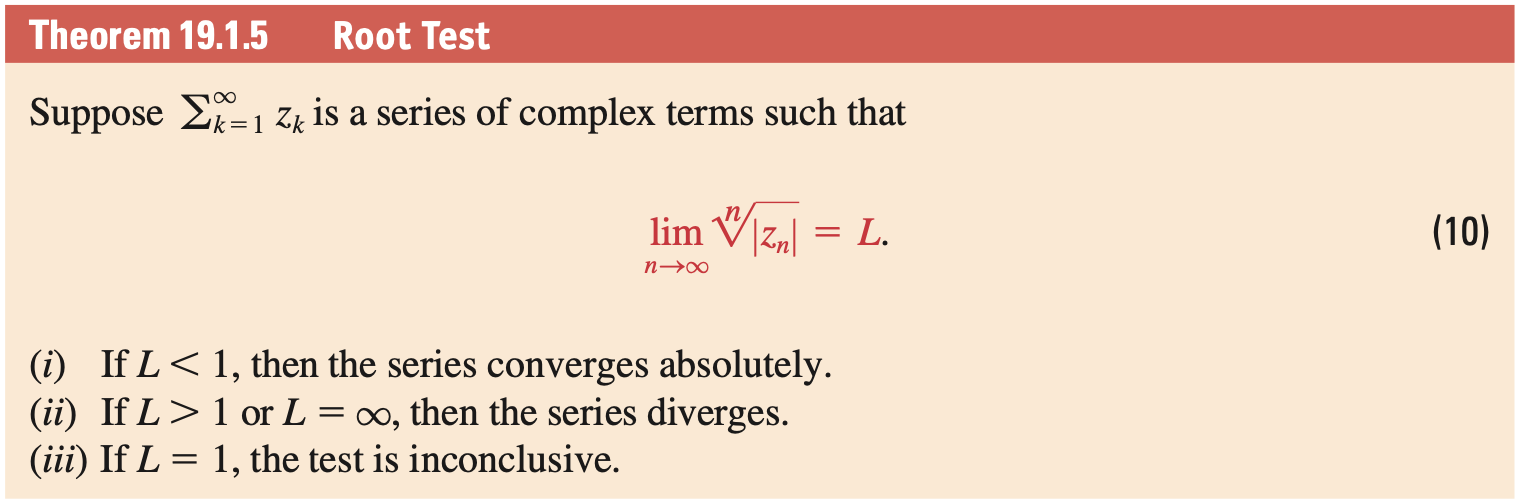
\includegraphics[width=\textwidth]{root-test}
\end{figure}

\begin{itemize}
  \item An infinite series of the form \[\sum_{k = 0}^\infty a_k (z - z_0)^k = a_0 + a_1 (z - z_0) + a_2 (z - z_0)^2 + \cdots\] where the coefficients $a_k$ are complex constants is called a \textbf{power series} in $z - z_0$. The power series is said to be \textbf{centred at $\boldsymbol{z_0}$}, and the complex point $z_0$ is referred to as the \textbf{centre} of the series.

  \item Every complex power series has a \textbf{radius of convergence $\boldsymbol{R}$} where $R$ is a real number. The power series converges for all $z$ within the \textbf{circle of convergence} $|z - z_0| < R$ and diverges for $|z - z_0| > R$. The series may converge at some, all, or none of the points on the actual circle of convergence.

  \item For a power series \[\sum_{k = 0}^\infty a_k (z - z_0)^k\] the ratio test depends only on the coefficients $a_k$. If \begin{enumerate}
          \item $\lim_{n \rightarrow \infty} \left| \frac{a_{n + 1}}{a_n} \right| = L \ne 0$, the radius of convergence is $R = 1 / L$;

          \item $\lim_{n \rightarrow \infty} \left| \frac{a_{n + 1}}{a_n} \right| = 0$, the radius of convergence is $\infty$;

          \item $\lim_{n \rightarrow \infty} \left| \frac{a_{n + 1}}{a_n} \right| = \infty$, the radius of convergence is $R = 0$.
        \end{enumerate}
\end{itemize}

\subsection{Taylor Series}

\begin{itemize}
  \item A power series $\sum_{k = 1}^\infty a_k (z - z_0)^k$ has a radius of convergence $R$. For each complex number $z$ within the circle of convergence, when substituted into the power series it converges to a unique value $L$. This defines a function $f$ that maps each $z$ to its corresponding $L$.
\end{itemize}

\begin{figure}[H]
  \centering
  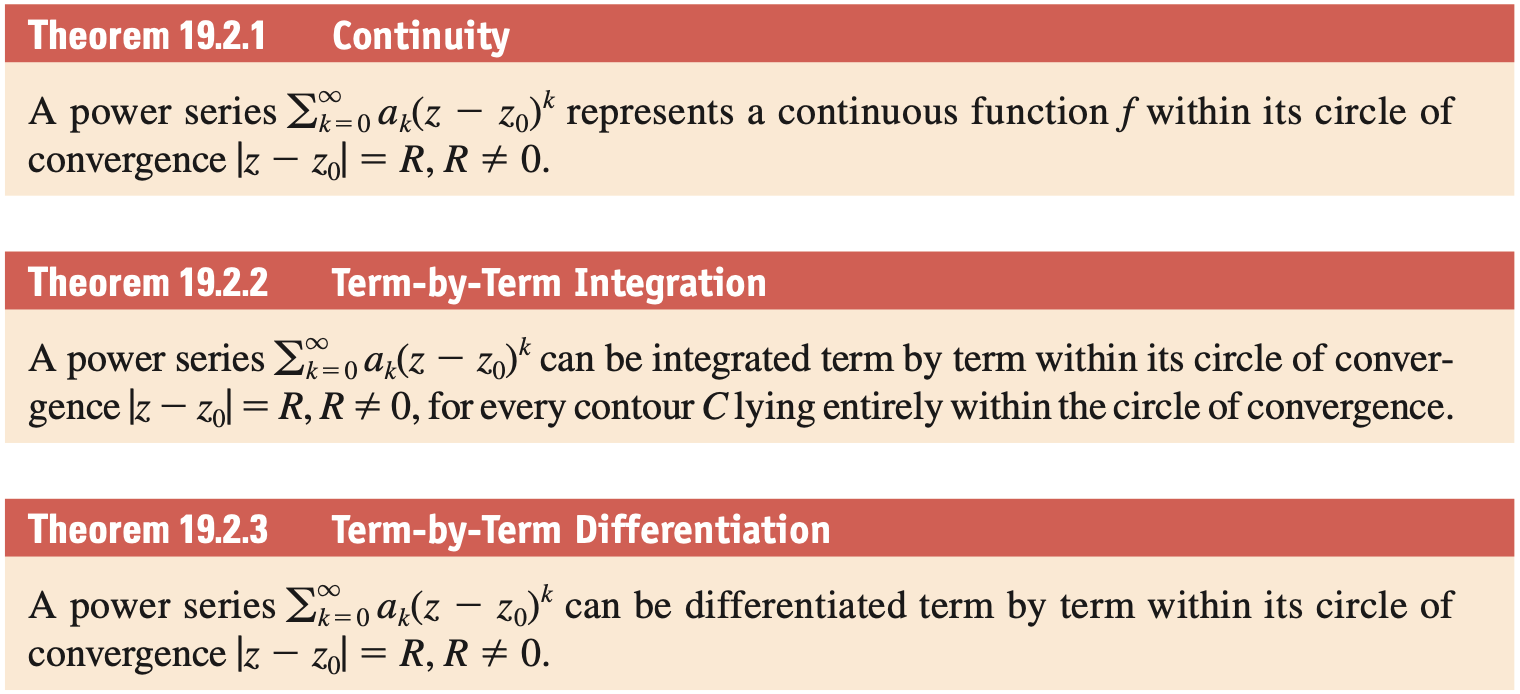
\includegraphics[width=\textwidth]{power-series-function-properties}
\end{figure}

\begin{figure}[H]
  \centering
  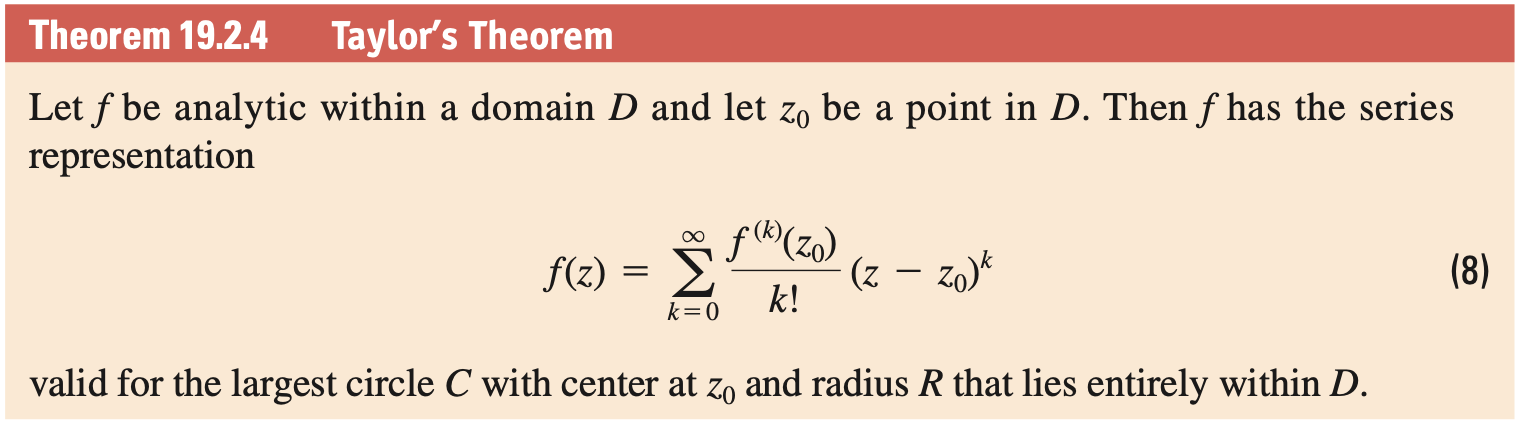
\includegraphics[width=\textwidth]{taylors-theorem}
\end{figure}

\begin{itemize}
  \item The radius of convergence of a Taylor series is the distance from the centre $z_0$ to the nearest isolated singularity: a point at which the series fails to be analytic but is analytic at all points in some neighborhood of the point.
\end{itemize}

\subsection{Laurent Series}

\begin{itemize}
  \item If a complex function $f$ fails to be analytic at a point $z = z_0$, then this point is said to be a \textbf{singularity} or a \textbf{singular point} of the function.

  \item Suppose $z = z_0$ is a singularity of a complex function $f$. It is said to be an \textbf{isolated singularity} if there exists some \textbf{deleted neighborhood}, or \textbf{punctured open disk}, $0 < |z - z_0| < R$ of $z_0$ in which $f$ is analytic.

  \item A singular point $z = z_0$ of a complex function $f$ is said to be \textbf{nonisolated} if every neighborhood of $z_0$ contains at least one singularity of $f$ other than $z_0$.
\end{itemize}

\begin{figure}[H]
  \centering
  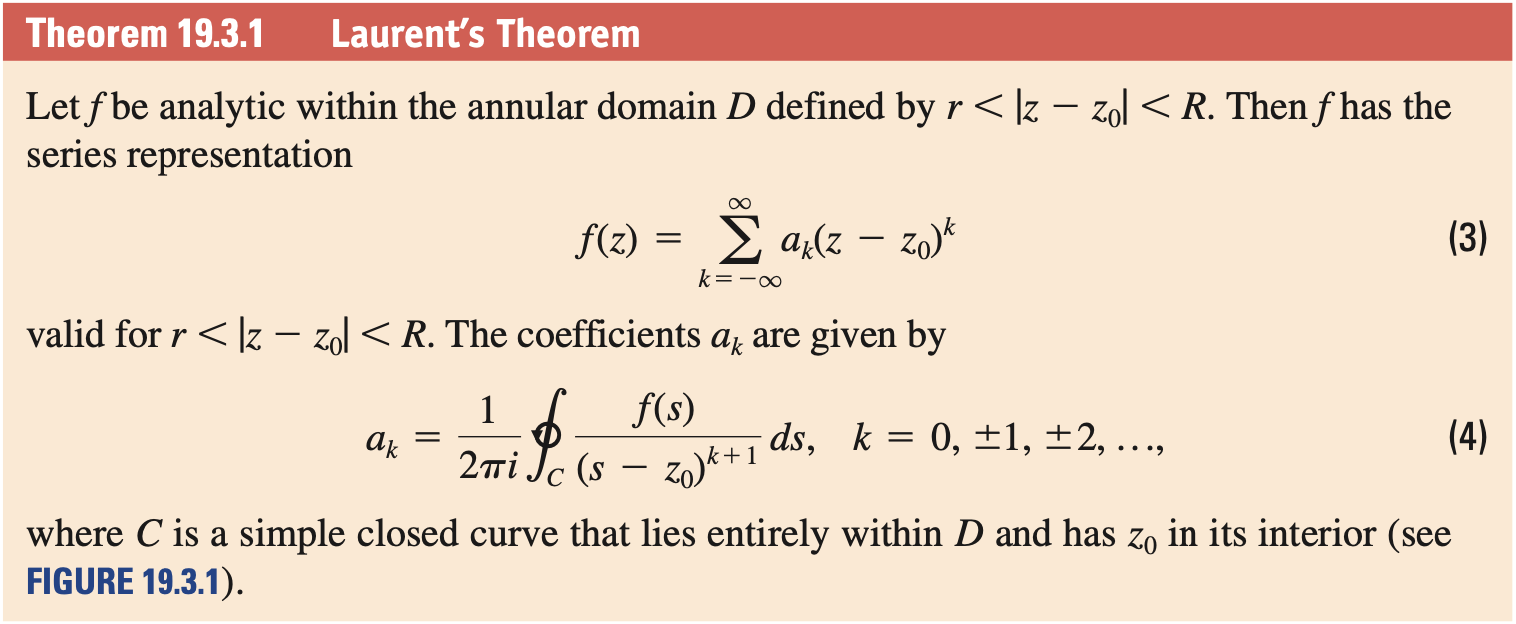
\includegraphics[width=\textwidth]{laurents-theorem}
\end{figure}

\begin{itemize}
  \item Under Laurent's theorem, the part of $f(z)$ with negative powers of $z - z_0$ is called the \textbf{principle part} and the part with positive powers is called the \textbf{analytic part}.

  \item The coefficient formula of theorem 19.3.1 isn't used often. Generally $f$ is decomposed into functions for which the series are known (e.g. $\cos z$, $e^z$, etc.), and those series are combined to find the Laurent series.
\end{itemize}

\subsection{Zeroes and Poles}

\begin{itemize}
  \item An isolated singularity $z = z_0$ can be categorised based on the number of terms contained in the principal part of its Laurent expansion (the part with negative powers).

        \begin{itemize}
          \item If the principal part is zero, i.e. the Laurent expansion consists only of parts with nonnegative powers, then $z = z_0$ is called a \textbf{removable singularity}.

          \item If the principal part contains a finite number of nonzero terms, then $z = z_0$ is called a \textbf{pole}. If the last nonzero coefficient of the principal part is $a_{-n}, n \ge 1$ then we say that $z = z_0$ is a \textbf{pole of order $\boldsymbol{n}$}. A pole of order $1$ is called a \textbf{simple pole}.

          \item If the principal part contains infinitely many nonzero terms, then $z = z_0$ is called an \textbf{essential singularity}.
        \end{itemize}
\end{itemize}

\begin{figure}[H]
  \centering
  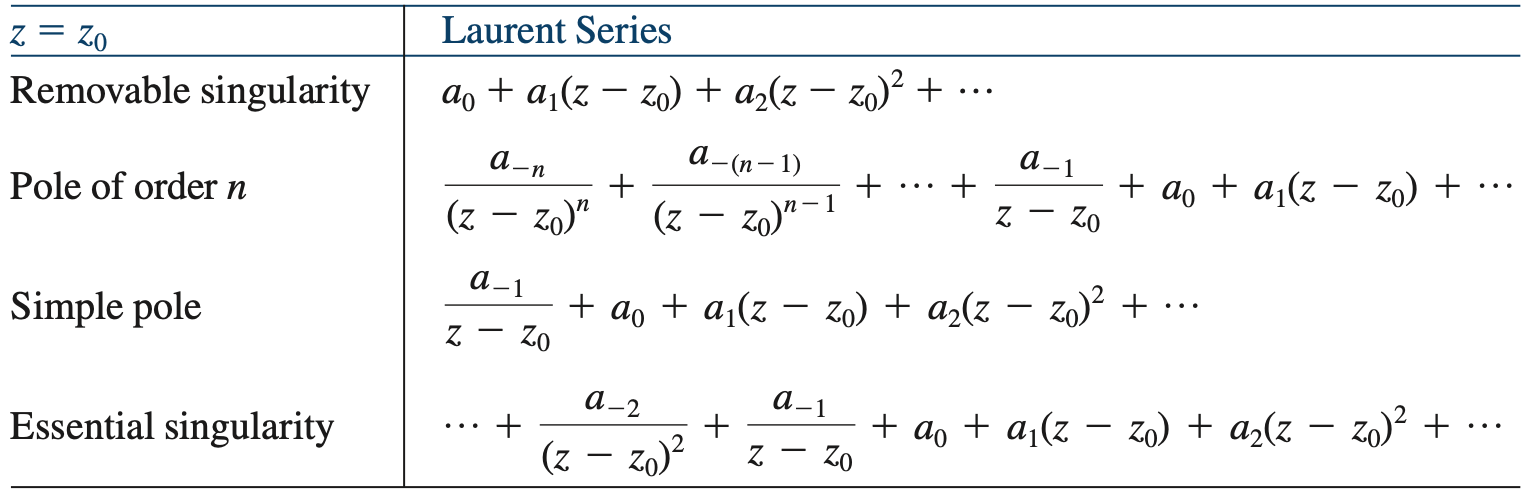
\includegraphics[width=\textwidth]{classification-of-isolated-singular-points}
\end{figure}

\begin{itemize}
  \item A point $z_0$ is said to be a \textbf{zero} of a function $f$ if $f(z_0) = 0$.

  \item A point $z_0$ is said to be a \textbf{zero of order $\boldsymbol{n}$} of a function $f$ if $f(z_0) = 0,\ f'(z_0) = 0,\ \ldots,\ f^{(n - 1)}(z_0) = 0$ but $f^{(n)}(z_0) \ne 0$.
\end{itemize}

\begin{figure}[H]
  \centering
  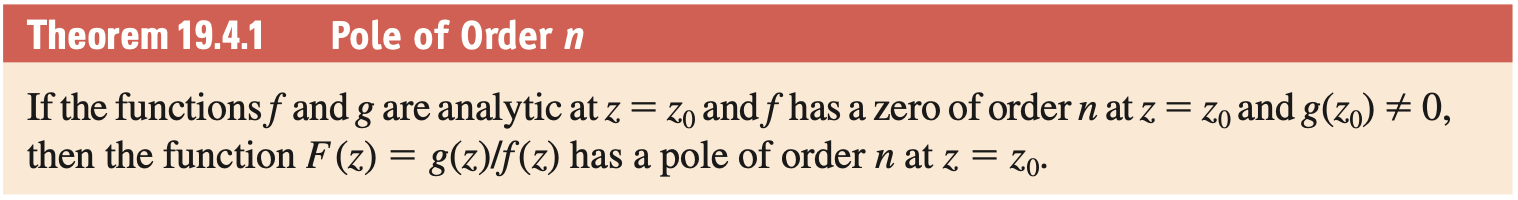
\includegraphics[width=\textwidth]{pole-of-order-n}
\end{figure}

\begin{itemize}
  \item Theorem 19.4.1 can sometimes be used to determine the poles of a function by inspection, e.g. in \[F(z) = \frac{2 z + 5}{z - 1}\] the denominator has a zero of order $1$ at $z = 1$ and the numerator is nonzero at that point so $F$ has a simple pole at $z = 1$.
\end{itemize}

\end{document}